\section{Actividad 1: Corriente de Saturación $I_{DSS}$}

\subsection{Simulación}

Para la primera simulacion vamos a implementar el siguiente circuito al simulador (LTSpice).
Resaltamos que en nuestro caso usamos el JFET MPF102, por lo cual añadimos una resistencia al drenador para proteger el elemento, dicha resistencia es de 510$\Omega$. Por lo que la añadiremos de ahora en adelante a las simulaciones para ser mas precisas.

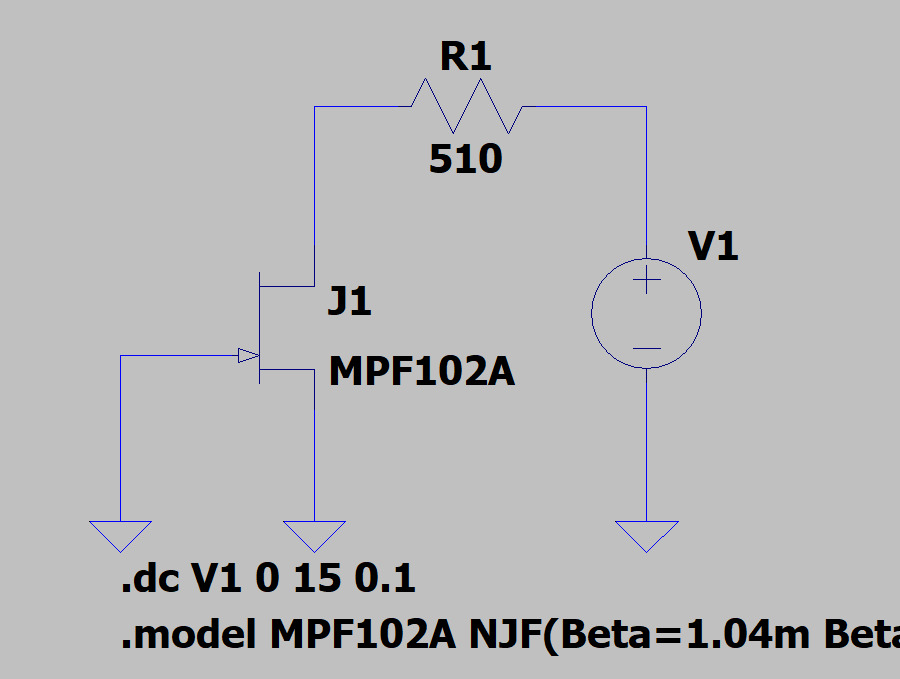
\includegraphics[width=6cm]{./imagenes/Circ1.png}

Observando el comportamiento de $I_{DS}$ con respecto a $V_{DS}$, obtenemos la siguiente gráfica:

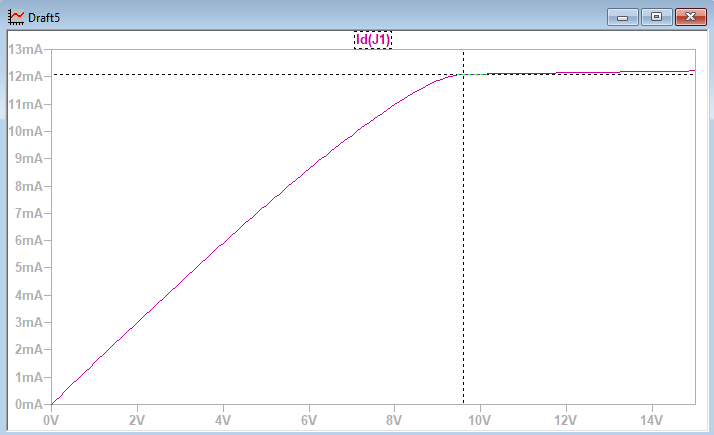
\includegraphics[width=8cm]{./imagenes/Sim1.png}

\subsection{Laboratorio}

\paragraph{Instrumental y Materiales}
\begin{itemize}
    \item Multimetro UNI-T UT89X
    \item Transistor JFET MPF102
    \item Resistor de 510$\Omega$
    \item Fuente de alimentación
\end{itemize}

\paragraph{Procedimiento:}

Para la realizacion de la actividad implementamos el circuito mostrado en la siguiente imagen, e hicimos variar el voltaje de la fuente desde 0 hasta 15V, punto en el que consideramos que el JFET mantiene su corriente constante. Los saltos medidos fueron impresisos para ver que ocurria en cada nivel de voltaje distinto hasta llegar a los 15V mencionados anteriormente.


Ejemplo de medición a 3V:

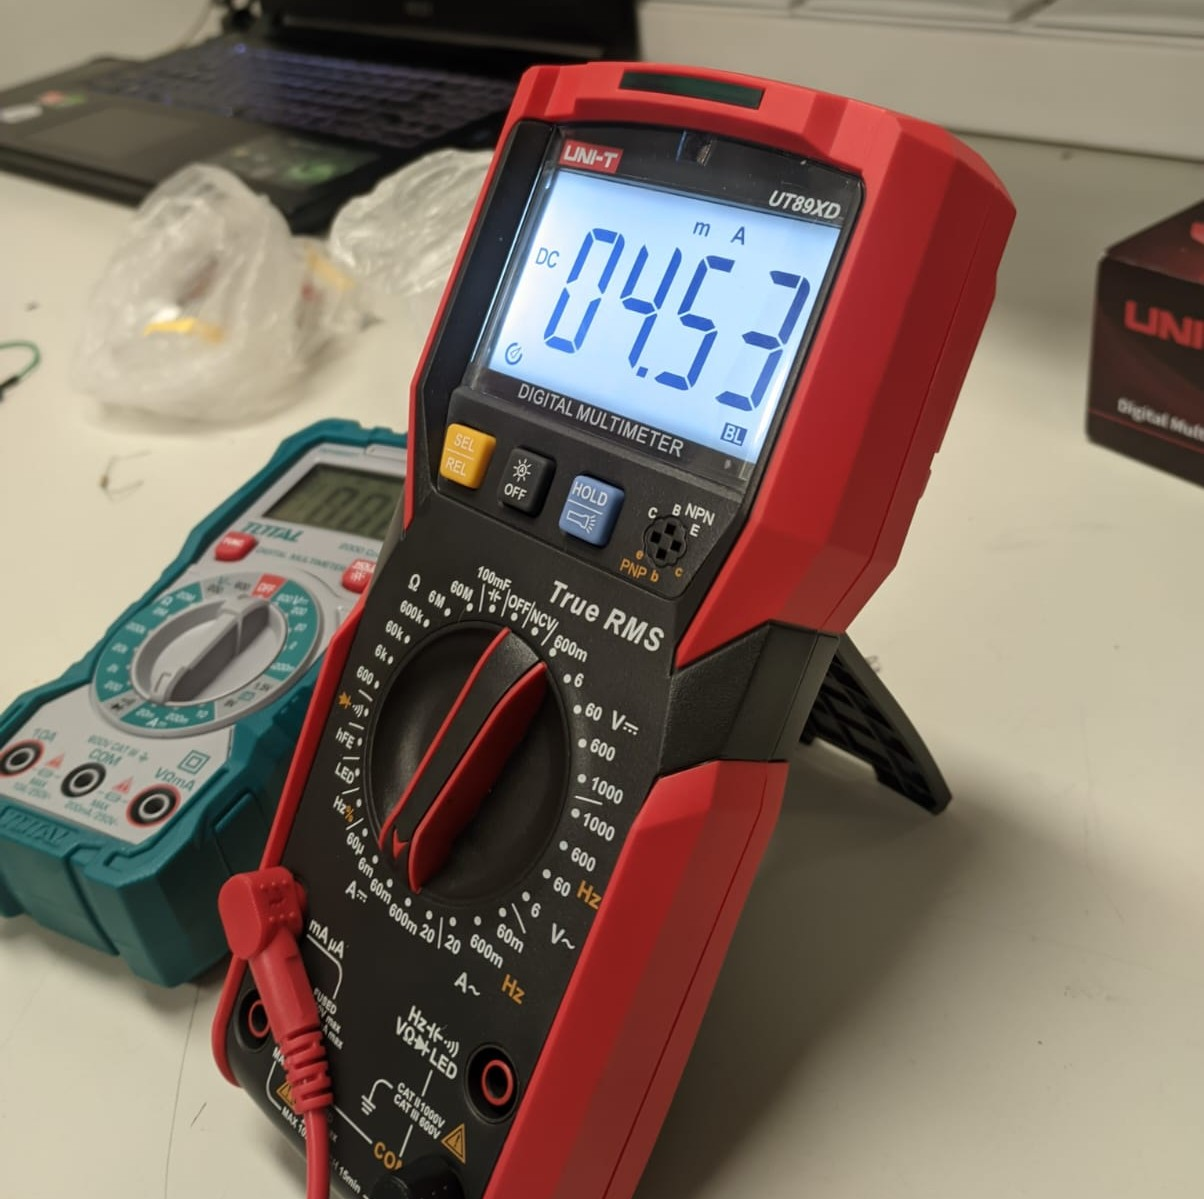
\includegraphics[width=6cm]{./imagenes/Res1.jpg}

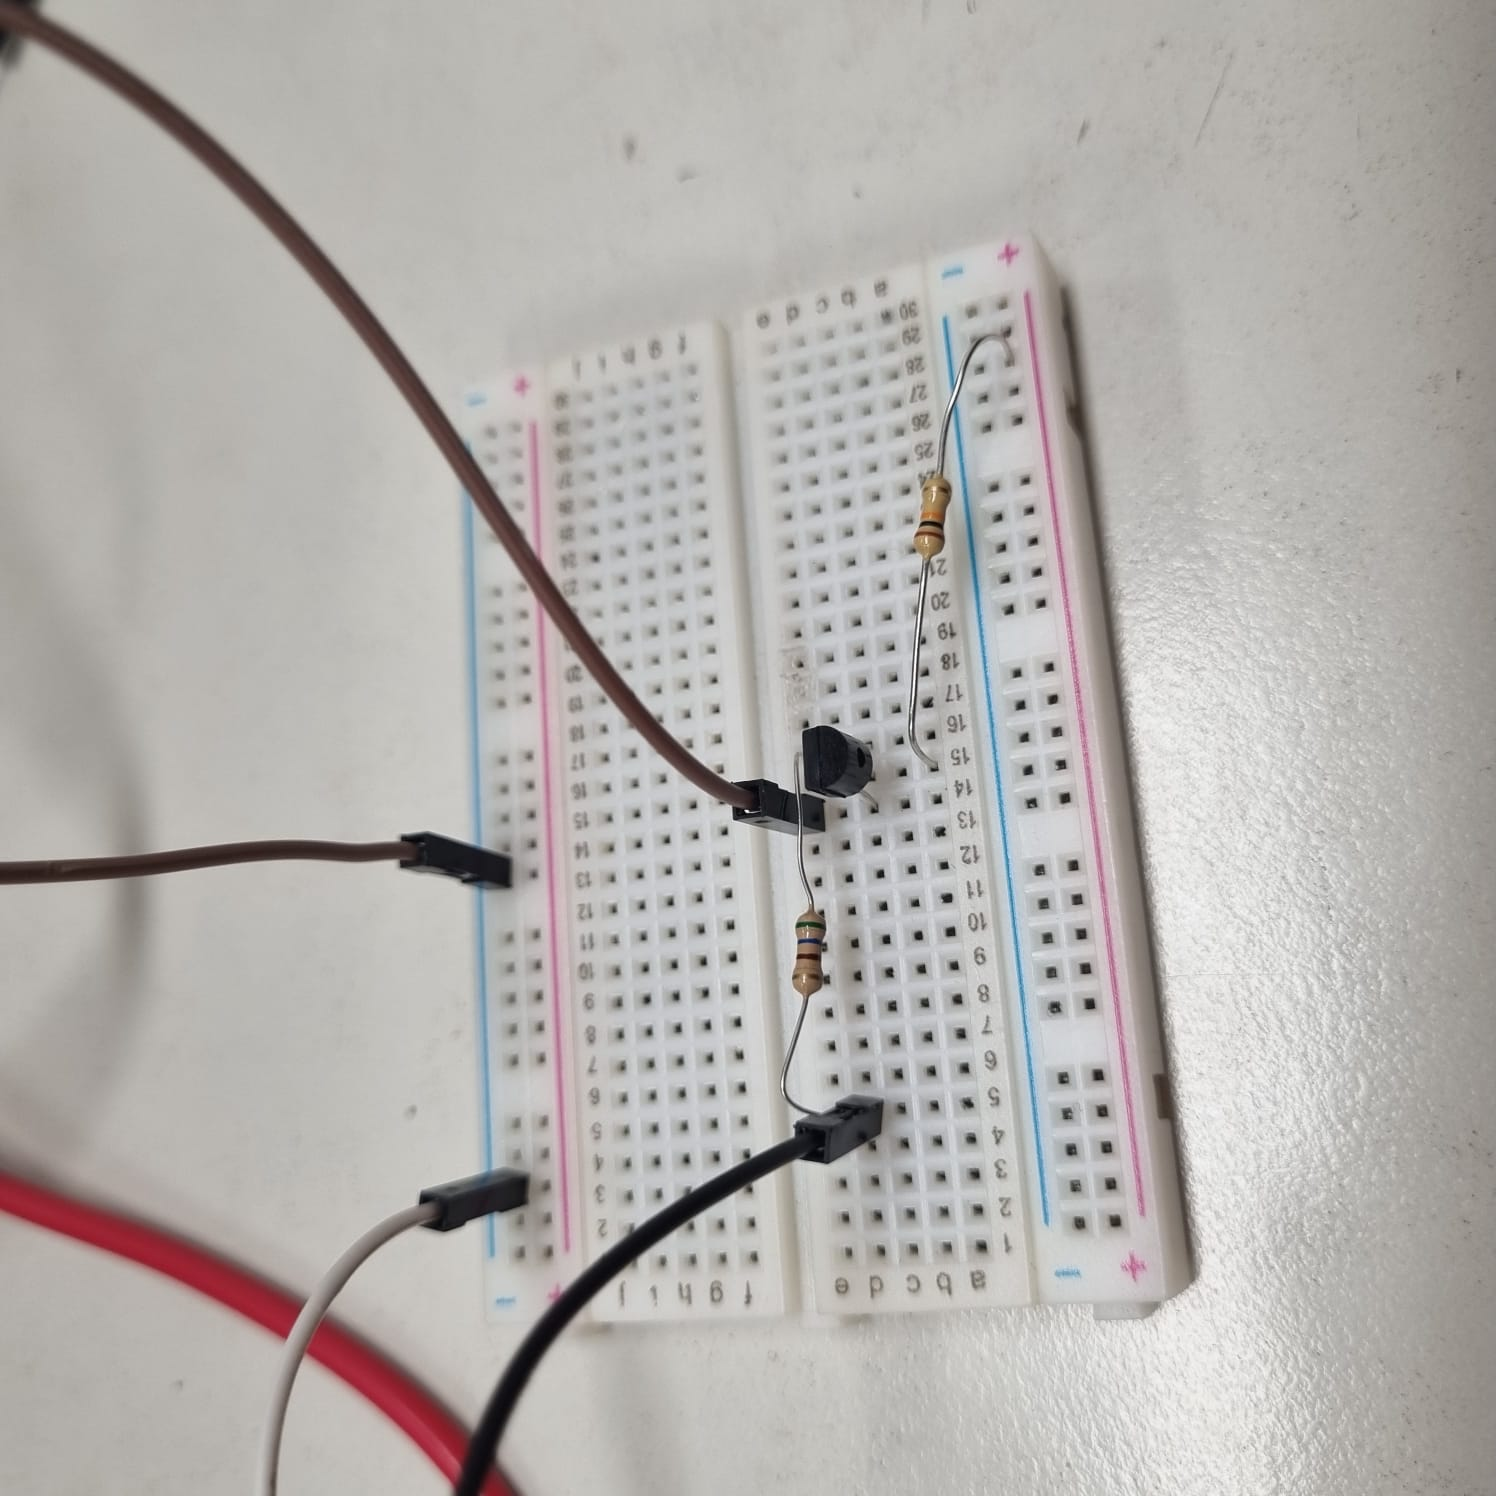
\includegraphics[width=6cm]{./imagenes/Lab1.jpg}


\begin{table}[ht]
\resizebox{6cm}{!}{%
\begin{tabular}{|l|l|}
\hline
\rowcolor[HTML]{FFCE93} 
$V_{DS}$ & $I_D$     \\ \hline
$150mV$  & $0,210mA$ \\ \hline
$1V$     & $1,61mA$  \\ \hline
$1,5V$   & $2,43mA$  \\ \hline
$2V$     & $3,2mA$   \\ \hline
$4V$     & $5,36mA$  \\ \hline
$6V$     & $6,48mA$  \\ \hline
$8V$     & $7,34mA$  \\ \hline
$10V$    & $8mA$     \\ \hline
$14,8V$  & $9,56mA$  \\ \hline
\end{tabular}
}
\end{table}

\vspace{0.1cm}

\subsection{Conclusión}

Podemos ver que el valor de $I_{DSS}$ es 9,56, lo cual difiere con el obtenido en la hoja de datos el cual es de 20mA, pero esto se debe a dos factores.\\
El primero es que la calidad del JFET seleccionado no es muy buena, y por ello hay diferencias en los valores.\\
Y la segunda es que para proteccion del elemento se le añadio la resistencia mencionada anteriormente, lo cual hace menor la corriente de drenaje.